\newpage
\section{Cacher du texte dans un fichier texte en pratique}
Pour la pratique, il faut retrouver les caractères zero-width pour pouvoir les convertir. Pour cela, il y a 2 manières de faire : Soit parcourir le fichier à la recherche du premier caractère zero width (ce que l'on va faire pour notre implémentation), soit stocker la taille de la donnée cachée en binaire sur les 8 derniers caractères zero-width du fichier.

\subsection{Encodage}
Les caractères zero-width n'étant pas supportés par le C, il faut inclure une librairie pour faire les conversions UTF-8 unicode. Pour cela, j'utilise la librairie wchar.h.
\newline
Il nous faut ensuite choisir 2 caractères zero-width pour représenter le 1 et 0 binaire :
\newline
\begin{lstlisting}
wchar_t zwnj=0x200C; //zero-width non joiner represents 1
wchar_t zws=0x200B; // zero-width space represents 0
\end{lstlisting}
On crée notre file descriptor vers le fichier qui va stocker notre message caché :
\newline
\begin{lstlisting}
textinfos.txtPtr=fopen(textinfos.path, "rw+");
    if(textinfos.txtPtr==NULL){
        printf("Unable to open file. Check if the file exists"
               " and that it was correctly specified in the command.");
        return 1;
    }
\end{lstlisting}
Ensuite, on va convertir le texte à encoder en binaire et stocker chacun des bits dans un buffer de unsigned char (plus petite valeur adressable avec des valeurs allant de 0 à 255).
\newline
\begin{lstlisting}
int fillTxtBuffer(const char * txt){
    textinfos.txtBuff = (unsigned char *) malloc(sizeof(unsigned char) * strlen(txt)*8);
    for(unsigned i=0; i<strlen(txt); i++){
        char currentChar=txt[i];
        for(int j=7; j>=0; j--){
            textinfos.txtBuff[(i*8)+j]=currentChar%2;
            currentChar/=2;
        }
    }

    textinfos.size=strlen(txt)*8;

    return 0;
}
\end{lstlisting}
On place le curseur de notre pointeur de fichier à la fin du fichier.
\newline
\begin{lstlisting}
fseek(textinfos.txtPtr, -1, SEEK_END);
\end{lstlisting}
On crée un fonction qui va convertir nos bits de notre buffer texte en caractères zero-width et les ajouter à notre fichier.
\newline
\begin{lstlisting}
void addToFile(char bin){
    if(bin==1){
        fputwc(zwnj, textinfos.txtPtr);
    }else{
        fputwc(zws, textinfos.txtPtr);
    }
}
\end{lstlisting}
Et enfin, on va boucler sur chacun des bits du buffer texte et appeler la fonction qui va convertir les bit du buffer et écrire ces caractères zero-width.
\begin{lstlisting}
for(unsigned i=0; i<textinfos.size; i++){
        addToFile(textinfos.txtBuff[i]);
    }
\end{lstlisting}

\subsection{Utilisation du script pour l'encodage}
Executer la section build du Makefile pour la compilation et l'édition des liens :
\begin{lstlisting}
make build
> gcc -g -Wall -o steganography main.o zwnj-zws.o lsb.o -lm -lpng -lz
\end{lstlisting}

Exécuter l'éxécutable généré en lui passant le type de stéganographie (zero-width), l'action(encode), le chemin du fichier qui va stocker la donnée et le texte qui va être caché.
\begin{lstlisting}
./steganography zero-width encode /home/noedelcroix/Documents/SYSG5/code/supports/test.txt Hello world
> Finished encoding
\end{lstlisting}
\subsection{Décodage}
Pour commencer, on crée de nouveau nos variables contenant nos zero-width characters.
\newline
\begin{lstlisting}
wchar_t zwnj=0x200C; //zero-width non joiner represents 1
wchar_t zws=0x200B; // zero-width space represents 0
\end{lstlisting}
On crée un file descriptor en lecture vers le fichier stockant les données cachées.
\newline
\begin{lstlisting}
textinfos.txtPtr=fopen(textinfos.path, "r");
\end{lstlisting}
On parcoure le fichier texte jusqu'à trouver le premier caractère zero-width.
\begin{lstlisting}
wchar_t val;
    val=fgetwc(textinfos.txtPtr);
    while(val!=zwnj && val!=zws && !feof(textinfos.txtPtr)){
        val=fgetwc(textinfos.txtPtr);
    }
\end{lstlisting}
Et enfin, on lit les caractères zero-width du fichier, on les convertit en binaire (avec la fonction ), on crée un char en groupant ces bits par 8 et on les retourne dans stdout.
\begin{lstlisting}
unsigned counter=7;
    char currentChar=pow(2, counter)*convertZw(val);
    while(!feof(textinfos.txtPtr) && (val==zwnj || val==zws)){
        counter--;
        val=fgetwc(textinfos.txtPtr);
        currentChar+=pow(2, counter)*convertZw(val);
        if(counter==0){
            printf("%c", currentChar);
            counter=8;
            currentChar=0;
        }
    }
\end{lstlisting}

Fonction convertZw :
\begin{lstlisting}
unsigned convertZw(const wchar_t val){
    return val==zwnj;
}
\end{lstlisting}

\subsection{Utilisation du script pour le décodage}
Executer la section build du Makefile pour la compilation et l'édition des liens :
\begin{lstlisting}
make build
> gcc -g -Wall -o steganography main.o zwnj-zws.o lsb.o -lm -lpng -lz
\end{lstlisting}

Exécuter l'éxécutable généré en lui passant le type de stéganographie (zero-width), l'action(decode) et le chemin du fichier qui contient la donnée cachée.
\begin{lstlisting}
./steganography zero-width decode /home/noedelcroix/Documents/SYSG5/code/supports/test.txt Hello world
> Finished decoding
\end{lstlisting}
\subsection{Résultat}
Comparons le contenu du fichier avant et après.
\newline
Avant : 
\newline
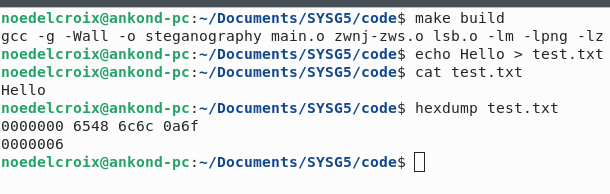
\includegraphics[width=1\textwidth]{img/resultat_before_zero-width.png}
Commande encodage :
\begin{lstlisting}
./steganography zero-width encode $(pwd)/test.txt "Ceci est un message secret."
\end{lstlisting}
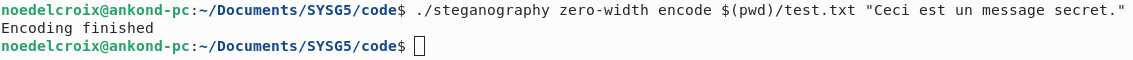
\includegraphics[width=1\textwidth]{img/resultat_commande_zero-width.png}
\newline
Après:
\newline
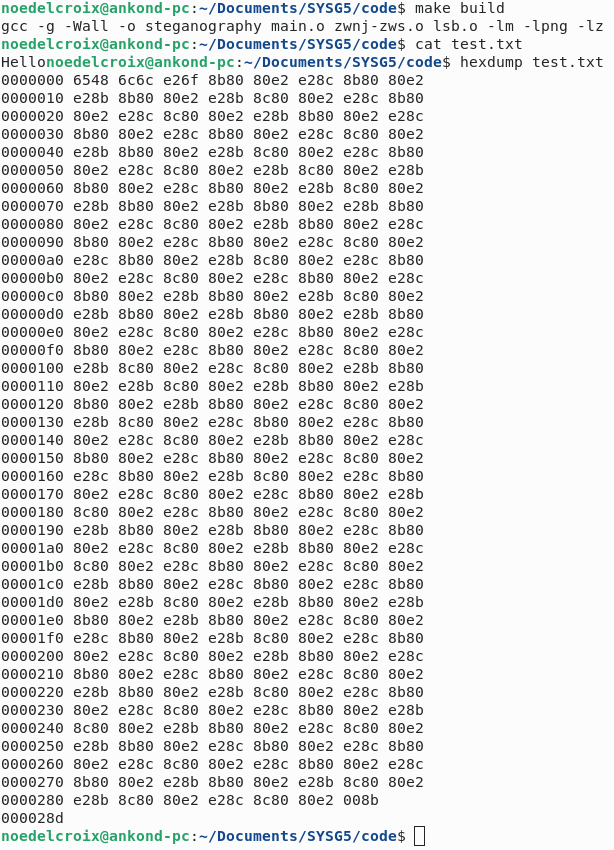
\includegraphics[width=1\textwidth]{img/resultat_after_zero-width.png}
Commande décodage :
\begin{lstlisting}
./steganography zero-width decode $(pwd)/test.txt
\end{lstlisting}
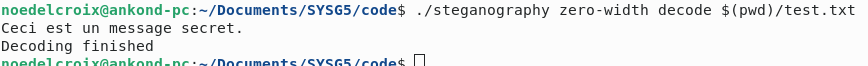
\includegraphics[width=1.3\textwidth]{img/resultat_commande_decodage_zero-width.png}
On remarque qu'après encodage du message caché, les données sont invisibles au niveau de l'interprétation des caractères unicodes. "Hello" apparait bien dans les 2 cas (avant et après encodage), ni plus, ni moins.
\newline
Mais au niveau du contenu binaire, on voit que l'on a beacuoup plus d'octets. On a en fait 8 fois la taille du message encodé qui se sont rajoutés à la fin du fichier texte (ici 27*8 octets pour le message "Ceci est un message secret.").
\newline
les caractères UTF-8 étant codés sur minimum 2 octets (pouvant aller jusque 6 octets), le code UTF-8 du zero-width no joiner est donc 8b80 80e2 e28c et du zero-width space est 8b80 80e2 008b